\documentclass{article}
\usepackage{todonotes}
\usepackage[utf8]{inputenc}       % Encodage UTF-8
\usepackage[T1]{fontenc}          % Meilleure gestion des polices
\usepackage[french]{babel}
\usepackage{report}
\usepackage{float}
%Marging
\usepackage[left=2.5cm,        % Équivalent à \oddsidemargin et \evensidemargin = -0.25in
    right=2.5cm,       % Marge droite (non spécifiée dans conference.sty, mais souvent symétrique)
    top=2.5cm,         % Équivalent à \topmargin = -0.25in
    bottom=2.5cm,      % Marge inférieure (non spécifiée dans conference.sty)
    columnsep=0.635cm, % Équivalent à \columnsep = 0.25in
    paperwidth=21.59cm, % Largeur standard d'une page A4 (21 cm) ou Letter (21.59 cm)
    paperheight=27.94cm
    %showframe,
    ]{geometry}


% multicol
\usepackage{multicol}

% biblio

% figure
\usepackage{graphicx}

%caption
\usepackage{caption}

% itemize
\usepackage{enumitem}

\usepackage{booktabs}

\usepackage{csvsimple}  
\usepackage[sorting=none,backend=biber]{biblatex}
\usepackage[colorlinks=true, linkcolor=red]{hyperref}  % pour liens cliquables
\usepackage[en-US]{datetime2}
\usepackage{csquotes}                 % Pour les citations complexes
\addbibresource{reference.bib}


\title{FIRLT : Fault Injection in Rust with Lazart Tool}
\author{
        Timothe Baleras
        \\
        \smallskip
        Ensimag,UGA,Verimag
        \\
        \smallskip
        timothe.baleras@grenoble-inp.org \\
        \bigskip
        Supervised by: Laurent Mounier,Etienne Boespflug
        }
\date{\today}

\begin{document}
\twocolumn
\maketitle

\DTMsetdatestyle{ddmmyyyy}
{% Mosig student
\fbox{\parbox{0.9\linewidth}{\small I understand what plagiarism entails and I declare that this report is my own, original work.\\   Baleras timothe, \today\space and signature:\\ \vspace{0.5cm} }}
}

%---------------------------Introduction---------------------------
\section{Abstract}
%\textbf{The Rust programming language \cite{27RustMatsakis} is rapidly being adopted in safety- and security-critical software. Its compile-time guarantees, thanks to borrow checking and some other language constructs — exhaustive pattern matching, mandatory error handling through \texttt{Option} and \texttt{Result}, and automatic bounds check — eliminate entire classes of memory-safety vulnerabilities that have plagued C and C++ for decades.}

\textbf{Fault injection is a critical security concern that can cause hardware to malfunction or be exploited by attackers. Rust is not protected from fault injection, as most of its protections are made at compile time and can be faulted during runtime.
That is why tools like Lazart are essential for identifying faults and evaluating code—including C and Rust—to protect systems from such vulnerabilities.}

\textbf{In this study, we extend the tool Lazart \cite{Lazart2015} to support the Rust language by updating its LLVM backend in order to support the pipeline of \texttt{cargo} and \texttt{rustc}, and by adding a new attack model giving Lazart the ability to change the address of a pointer during execution. A new option has been added to the Lazart tool giving the ability to generate a control flow graph of the compiled code or its mutated version.
Finally, we ported the FISSC fault injection collection from C to Rust and provided a more Rust-idiomatic version of the collection.
The results section covers the findings of FISSC and evaluates the impact of the new control flow graph generator. It highlights that Rust and C diverge both in design and in their approach to control flow by utilizing instructions typically reserved for pattern matching.}
\todo[inline]{Remade Abstract}
\section{Introduction}
\subsection{Fault injection}
In computer science, many types of faults can cause a system to behave unexpectedly.
Faults may occur during the development or execution of a program and can originate from the software, the hardware, or both.
Faults come in a wide variety: they can be syntax errors that cause the script to fail to compile, generated warnings, or crashes with an error during compilation.
Faults can be caused by human error, misconfigurations that were not anticipated, or malicious individuals exploiting security vulnerabilities.
One important type of fault is \textbf{fault injection}.
Fault injection has been around for a long time, and we found traces of papers dating from the 1970s, but they were never published; the oldest one published is from 1995 \cite{1_Segall1995}.
This fault can be caused by various techniques, including hardware, such as clock glitches \cite{15obermaier2017fuzzy,16korak2014effects}, voltage glitches \cite{11zussa2012investigation, 12zussa2014analysis, 13selmane2011security}, laser \cite{17selmke2016precise, 18dutertre2018laser}, or electromagnetic faults \cite{19dehbaoui2012injection, 20dehbaoui2012electromagnetic}, as well as software, such as Rowhammer \cite{14kim2014flipping}.
It can occur accidentally, for example due to cosmic rays, or deliberately by a mischievous individual; in the latter case, we talk about a fault injection attack.
To deal with fault injection, developers use several countermeasures \cite{dureuil2016,liu2025,Richter-Brockmann2021} or tools \cite{Arlat1990,Arribas2020,1_Segall1995,pensec2024} to protect their programs.
One such tool is called Lazart\cite{Lazart2015}. It is a multi-fault injection tool that mutates the code at the LLVM level in order to simulate the effects of fault injection attacks.

\subsection{Rust}

The Rust language is a recent language defined as a successor to C and C++;
while C/C++ have a lot of memory access bugs such as buffer overflows or data race issues.

Rust has stronger protection over memory access and concurrency over variables; variables are tracked with an element called the borrow checker that tracks the lifespan and ownership, as well as their access.
While the borrow checker protects against bad access of data in the software program. 

The same cannot be said for hardware failure, which may cause some protections to be countered.

\todo[inline]{section 2.2 :Si tu veux plus parler du borrow-checker alors tu peux prendre l'exemple
   de Tommy (échange de pointeurs) du papier FDTC. Tu peux aussi faire réference à la section 4 qui détaille cet exemple ...,ref FDTC ?}

We can take the buffer overflows of a table rust protection as an example.
\texttt{rustc} will add a test on the code at compile time, to identify if you reading in or out the table, and will launch a pannic if it's outside the range of the table.
injected a faute at the moment of the condition can allow the program to read outside the table, and thus counter the protection set by Rust language itself.

An other example, is the change pointer fault. It is explained in the subsection \ref{subsection:Change Pointer fault model}.

\subsection{Contribution}
 
The purpose of this report is to show how Rust differs from C and C++ regarding offensive fault injection.
To answer that, there are two different parts:

\begin{itemize}
\item \textbf{Extend Lazart to support Rust}: discussed in section \ref{Section:Rust ported}, this shows the instructions that have to be added in order to analyze Rust programs without losing attacks. In addition, we also discuss the change pointer fault in this section.
\item \textbf{Porting the FISSC benchmark to Rust}: this point discusses FISSC (Fault Injection and Simulation Secure Collection) \cite{dureuil2016}. We analyze two programs of FISSC in Rust and C and compare them to each other. See section \ref{Section:FISSC}
\end{itemize}

The report is organized as follows. Section \ref{Section:Related_work} presents the Rust programming language, related work concerning Rust and fault injection, and the tool Lazart. Section \ref{Section:Rust ported} describes the extension of Lazart to support the Rust language and the addition of a new attack model for C and Rust languages. Section \ref{Section:CFG} presents a new option of the Lazart tool giving the possibility to generate a control flow graph (CFG). Section \ref{Section:FISSC} shows the comparison made on the FISSC benchmark and a Rust implementation designed to match the C implementation's attack surface. Section \ref{Section:result section} shows results for the FISSC comparison of a Rust implementation, and findings that were produced from control flow graph analysis. And finally, Section \ref{section:Conclusion} summarizes and proposes some perspectives to this work.

%Originally, Lazart only supported C code, but support for Rust is now being implemented. 
%In previous work, a countermeasure benchmark was implemented and evaluated in C \cite{dureuil2016}.

%The purpose of this study is to evaluate Fault injection on Rust code and to compare its results with the ones obtained with C on a representative benchmark.
%Another question addressed in this study, whether there is a way to protect fault injection countermeasures from compiler optimisations, and how much effectiveness remains after the optimisation.



\section{Related work}
In this section we talk about related work and a description of lazart tool.
\subsection{Fault injection}
Fault injection is an old, well-studied attack models in security and cryptology that can be created at hardware or software level\cite{liu2025}.
While multiple methods exist multiple methods to simulate fault injection, one approach involves hardware-based techniques, such as \cite{Richter-Brockmann2021,Arribas2020}. 
Another method to simulate fault injection is using software tools \cite{Lazart2015,Riviere2014}. 
One sush software tool is called Lazart \cite{Lazart2015}.
A countermeasure benchmark, developed using the Lazart tool by several researchers, is FISSC \cite{dureuil2016}.  

While a few studies have been conducted on countermeasures in Rust \cite{21Kim2026ICCE,22Sini2025DATE} ,there is little research that has been conducted on comparing the results between C and Rust for countermeasures.

Furthermore, little research has been done on the effectiveness of the protecting of the countermesure from compiler optimisations.
We addressed this gap by highlighting the work of Sébastien Michelland \cite{23miche2025}.

\subsection{Lazart tools}
\label{subsec:Lazart}
\begin{figure*}
    \centering
    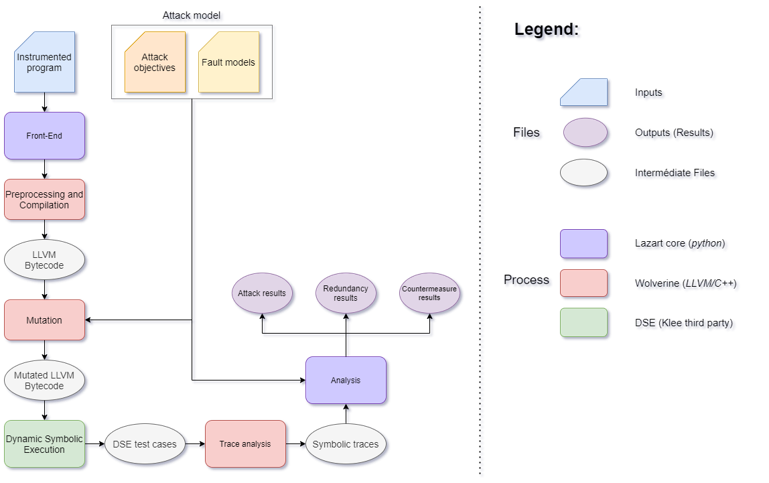
\includegraphics{image/lazart-arch.png}
    \caption{Lazart tool arkitecture}
    \label{figure_0:Lazart}
\end{figure*}

Lazart \cite{Lazart2015} is a high level fault injection tool.
Has been develop by Verimag since 2015.
It allows to identifying vulnerable paths in code and can be used to evaluate the accuracy of countermeasures against a given fault model and a security property.
Unlike other similar tools, Lazart is one of the few that are capable of performing multi-fault attacks.
Lazart is able to analyse C or C++ code by compiling it using the Clang compiler.
They use one of the features of Clang to generate LLVM bitecode (which is Intermediate code).\\
LLVM is a middle component of the compiler and is designed for compile-time, link-time and run-time optimisation.
The LLVM framework is run by Clang after the frontend pipeline is completed.

Lazart is composed of five step:
\begin{enumerate}[noitemsep,leftmargin=0em,wide]
\item Preprocessing and compilation of the input code.
\item Mutation of the code with Wolverine.
\item Dynamic-Symbolic Execution with KLEE \cite{24Cadar2008KLEEUA,25kleeseKLEE}.
\item Trace parsing from KLEE's outputs.
\item Analysis.
\end{enumerate}

Lazart can support 4 fault models:
\begin{itemize}[noitemsep,leftmargin=0em,wide]
    \item Test inversion (modification of the evaluation of a branch condition);
    \item data mutation (modification of the loaded values);
    \item instruction skip;
    \item Call another function (function switch);
\end{itemize}

\todo[inline]{under new section}

\subsection{Rust Language}
Rust is a general-purpose programming language which emphasizes performance, type safety, concurrency, and memory safety.
Rust has is first version released in 2006.
One of features of rust is the way hwo it handle the memory safety and concurrency of a program.
Unlike other language who use a garbage colector, Rust use a "barrow checker" that track the life spand of a variable as there owner.
And deal with data races. 

\subsubsection{Why using Rust ?}
We give several reason of using rust: 
\begin{itemize}
    \item Rust use the same LLVM as clang does in C/C++. So it make Rust compatible with lazart.
    \item Rust is a recent,still updated programming language.
    \item Rust is used for embeded system.
\end{itemize}

\subsubsection{The usage of no\_std}
One point that need to be explain on this reporte is the flag no\_std.
Using no\_std attribute stops the compiler from linking std into the crate, and only links core.
It limit :
\begin{itemize}
    \item Heap allocation.
    \item File I/O, threading, and networking.
    \item Many common traits and types (e.g., std::io::Error).
\end{itemize}

\todo[inline]{below new section}



%--------------------------Core------------------------------------
\section{Contribution}
%\todo[inline]{Add discovery of rust ralated problem in rust + Redo the contribut not enough clear + add feature readded (graph normal and mutated)}
\input{core/contribution.tex}

\section{result}
\todo[inline]{add devrait se remplir facilement en reprenant les résultats FDTC}
%\label{Section:result section}
In this section, we first present the results obtained for the \texttt{memcmps} code.\\
Next, we show the results for the \texttt{verify\_pin} code.\\
Finally, we discuss the findings related to the control-flow graph generated during the analysis.

%------------------------------------------------verify_pin-----------------------------------------------
\subsection{Verify pin}
This section presents the results for the \texttt{verifypin} test.

\begin{table*}[t]
\centering
\begin{tabular}{l|llll|llll|l}
Version    & \multicolumn{4}{c|}{Attacks} & \multicolumn{4}{c|}{Non-redundant attacks} & Countermeasures \\
           & 1F & 2F & 3F & 4F & 1F & 2F & 3F & 4F &                 \\
\hline
\hline
VP0        & 12 & 21  & 18  & 7    & 12 & 0  & 0   & 0   & $\emptyset$           \\
VP0 - rust & 8  & 20  & 20  & 10   & 8  & 0  & 0   & 0   & $\emptyset$           \\
\hline
VP1        & 12 & 21  & 18  & 7    & 12 & 0  & 0   & 0   & HB                    \\
VP1 - rust & 12 & 21  & 18  & 7    & 12 & 0  & 0   & 0   & HB                    \\
\hline
VP2        & 34 & 122 & 204 & 183  & 34 & 4  & 0   & 0   & HB+FTL                \\
VP2 - rust & 34 & 122 & 204 & 183  & 34 & 4  & 0   & 0   & HB+FTL                \\
\hline
VP3        & 35 & 122 & 204 & 183  & 35 & 4  & 0   & 0   & HB+FTL+INL            \\
VP3 - rust & 35 & 122 & 204 & 183  & 35 & 4  & 0   & 0   & HB+FTL+INL            \\
\hline
VP4        & 34 & 118 & 180 & 147  & 34 & 0  & 4   & 0   & FTL+INL+DPTC+PTCBK+LC \\
VP4 - rust & 34 & 118 & 180 & 147  & 34 & 0  & 4   & 0   & FTL+INL+DPTC+PTCBK+LC \\
\hline
VP5        & 0  & 80  & 644 & 2566 & 0  & 80 & 248 & 184 & HB+FTL+DPTC+DC        \\
VP5 - rust & 0  & 80  & 644 & 2566 & 0  & 80 & 248 & 184 & HB+FTL+DPTC+DC        \\
\hline
VP6        & 0  & 3   & 9   & 20   & 0  & 3  & 9   & 14  & HB+FTL+INL+DPTC+DT    \\
VP6 - rust & 0  & 3   & 9   & 20   & 0  & 3  & 9   & 20  & HB+FTL+INL+DPTC+DT    \\
\hline
VP7        & 1  & 2   & 8   & 13   & 1  & 2  & 8   & 13  & HB+FTL+INL+DPTC+DT+SC \\
VP7 - rust & 1  & 2   & 8   & 13   & 1  & 2  & 8   & 13  & HB+FTL+INL+DPTC+DT+SC
\end{tabular}
    \caption{Comparison of attacks between \texttt{verify\_pin} implementations \label{tbl:results-fissc-vp}}
\end{table*}

\noindent Table \ref{tbl:results-fissc-vp}: present the attacks identified by Lazart for the code C and Rust.
The column "Version" indicates the version of the program and the implementation language. 
The second to fifth columns correspond respectively to the number of attacks reported by Lazart for 1 fault to 4 faults.
Similarly, the next four columns present the number of \textit{non-redundant} attacks for 1 fault to 4 faults. 
The last column "Countermeasures" enumerates the protection used for each version (the protection are the same for version X, and it's Rust counterpart):
\begin{itemize}
        \item \textit{HB} : hardened boolean
        \item \textit{FTL} : fixed time loops
        \item \textit{INL} : inlined function
        \item \textit{DPTC} : try counter decremented first
        \item \textit{PTCBK} : try counter backup
        \item \textit{LC} : loop counter verification
        \item \textit{DC} : double call
        \item \textit{DT} : double test
        \item \textit{SC} : step counter
\end{itemize}

In the VP0 example, we observe 8 missing attacks when we compare to the C result. Since VP0 doesn't have hardened boolean, so it uses regular boolean, \texttt{rustc} reuse the branch condition in the \texttt{verify\_pin} function, through XOR operations, to compute its return value, reducing the number of observable injection points on that path. All the higher-order attacks are redundant with those 8 one fault attacks.

The \textit{redundancy analysis} regroups attacks that are variations of a simpler attack adding additional faults.

In the VP6 example, the non-redundant attacks count differs in 4-fault (while being the same without redundancy analysis) because \texttt{rustc} places some injection points earlier in the control flow. The IPs are therefore identified as the non-redundant ones, which changes the higher-order results.
%------------------------------------------------memcompare-----------------------------------------------
\subsection{memcmps}
\label{section:memcmps_result}
This section presents the results for the \texttt{memcmps} test.

\begin{table*}[t]
\centering
\begin{tabular}{l|llll|llll}
Version      & \multicolumn{4}{c|}{Attacks} & \multicolumn{4}{c}{Non-redundant attacks} \\
             & 1F & 2F & 3F & 4F & 1F & 2F & 3F & 4F \\
\hline
\hline
MCMPS1        & 16  & 32  & 28  & 8  & 16  & 0  & 0  & 0  \\
MCMPS1 - rust & 16  & 32  & 28  & 8  & 16  & 0  & 0  & 0  \\
\hline
MCMPS2        & 4  & 32  & 404  & 1400 & 4  & 32  & 322  & 194  \\
MCMPS2 - rust & 4  & 32  & 404  & 1400 & 4  & 32  & 322  & 194  \\
\hline
MCMPS3        & 4  & 32  & 216  & 2262   & 4  & 32  & 134  & 1468  \\
MCMPS3 - rust & 4  & 32  & 216  & 2262   & 4  & 32  & 134  & 1468  \\
\end{tabular}
\caption{Comparison of attacks between \texttt{memcmps} implementations \label{tbl:results-fissc-mcmp}}
\end{table*}

Table \ref{tbl:results-fissc-mcmp} indicates for each version and implementation language (first column "Version") the results obtained for 1 to 4 faults - as for Table \ref{tbl:results-fissc-vp}, the column "Attacks" shows attacks count while the "Non-redundant attacks" column shows the subset of non-redundant attacks.


Table \ref{tbl:results-fissc-mcmp} presents the attack found by Lazart for the code C and Rust.\\
Version 1 (V1) uses one mask and one call to \texttt{memcmp}.\\
Version 2 (V2) uses one mask and three calls to \texttt{memcmp}.\\
Version 3 (V3) uses two masks and four calls to \texttt{memcmp}.\\
Version 3 is also the one shown in Figure \ref{tbl:results-fissc-mcmp}.\\

As shown in Table \ref{tbl:results-fissc-mcmp}, the Rust implementation behaves exactly as the C implementation, showing the same result for 1 to 4 faults with a combination of TI and DL fault models.

%------------------------------------------------CFG-----------------------------------------------

       
\subsection{Control Flow Graph}
\label{subsection:result cfg}
We also observed some major differences in how Rust compiles compared to C.\\
The intermediate code generated by LLVM revealed that Rust optimises certain conditional blocks differently than C.\\

However, we noticed differences in the control-flow graphs generated by the two language versions of the code presented in this study.\\
Specifically, Rust transforms variables with two possible values—depending on the evaluation of a condition, into a \texttt{select} instruction rather than a branch instruction.
Similarly, Rust may use a \texttt{switch} instruction when a variable is compared to multiple values.
\section{Conclusion}
%\label{section:Conclusion}
The first point of the report was to port Rust language in lazart.Lazart is now capable of analising Rust program and be able to fault \texttt{select} and \texttt{switch} instruction.

On the second point of the article there is now the possible to generated control flow graph of the code generated.The code generated could be the mutated or from the compile program.The use of cfg show that \texttt{rustc} use \texttt{select} and \texttt{switch} rather then normal conditional bloc arkitecture.

And finally on the last section, show that we almost get the same attack fault between both language with \texttt{verify\_pin} and \texttt{memcmps}.
the minor different are cause by rust using the result of the condition with the help of xor to return the value in \texttt{verify\_pin} 0 and the lost of some attacks in the version 6 of \texttt{verify\_pin}, due to the attack not being in the same places than in C.
However it show that the rust ported in lazart is reliable and can be trusted.
Further more an idiomatic version of FISSC as been added, to be more closer of what a reel programmers in rust will have done.

Even if Successfull version of lazart working with rust there is still element to improve and issue to be fix, one of them would be the panic function that cause klee to fall in a infinite loop or the use of intrassic optimisation instruction (optimisation done at runtime) done by the LLVM.
 
%\end{multicols}
\onecolumn
\section{Reference}
\printbibliography[heading=none]



%\newpage
\section*{Apendix A}
\begin{figure}[ht]
    \centering
    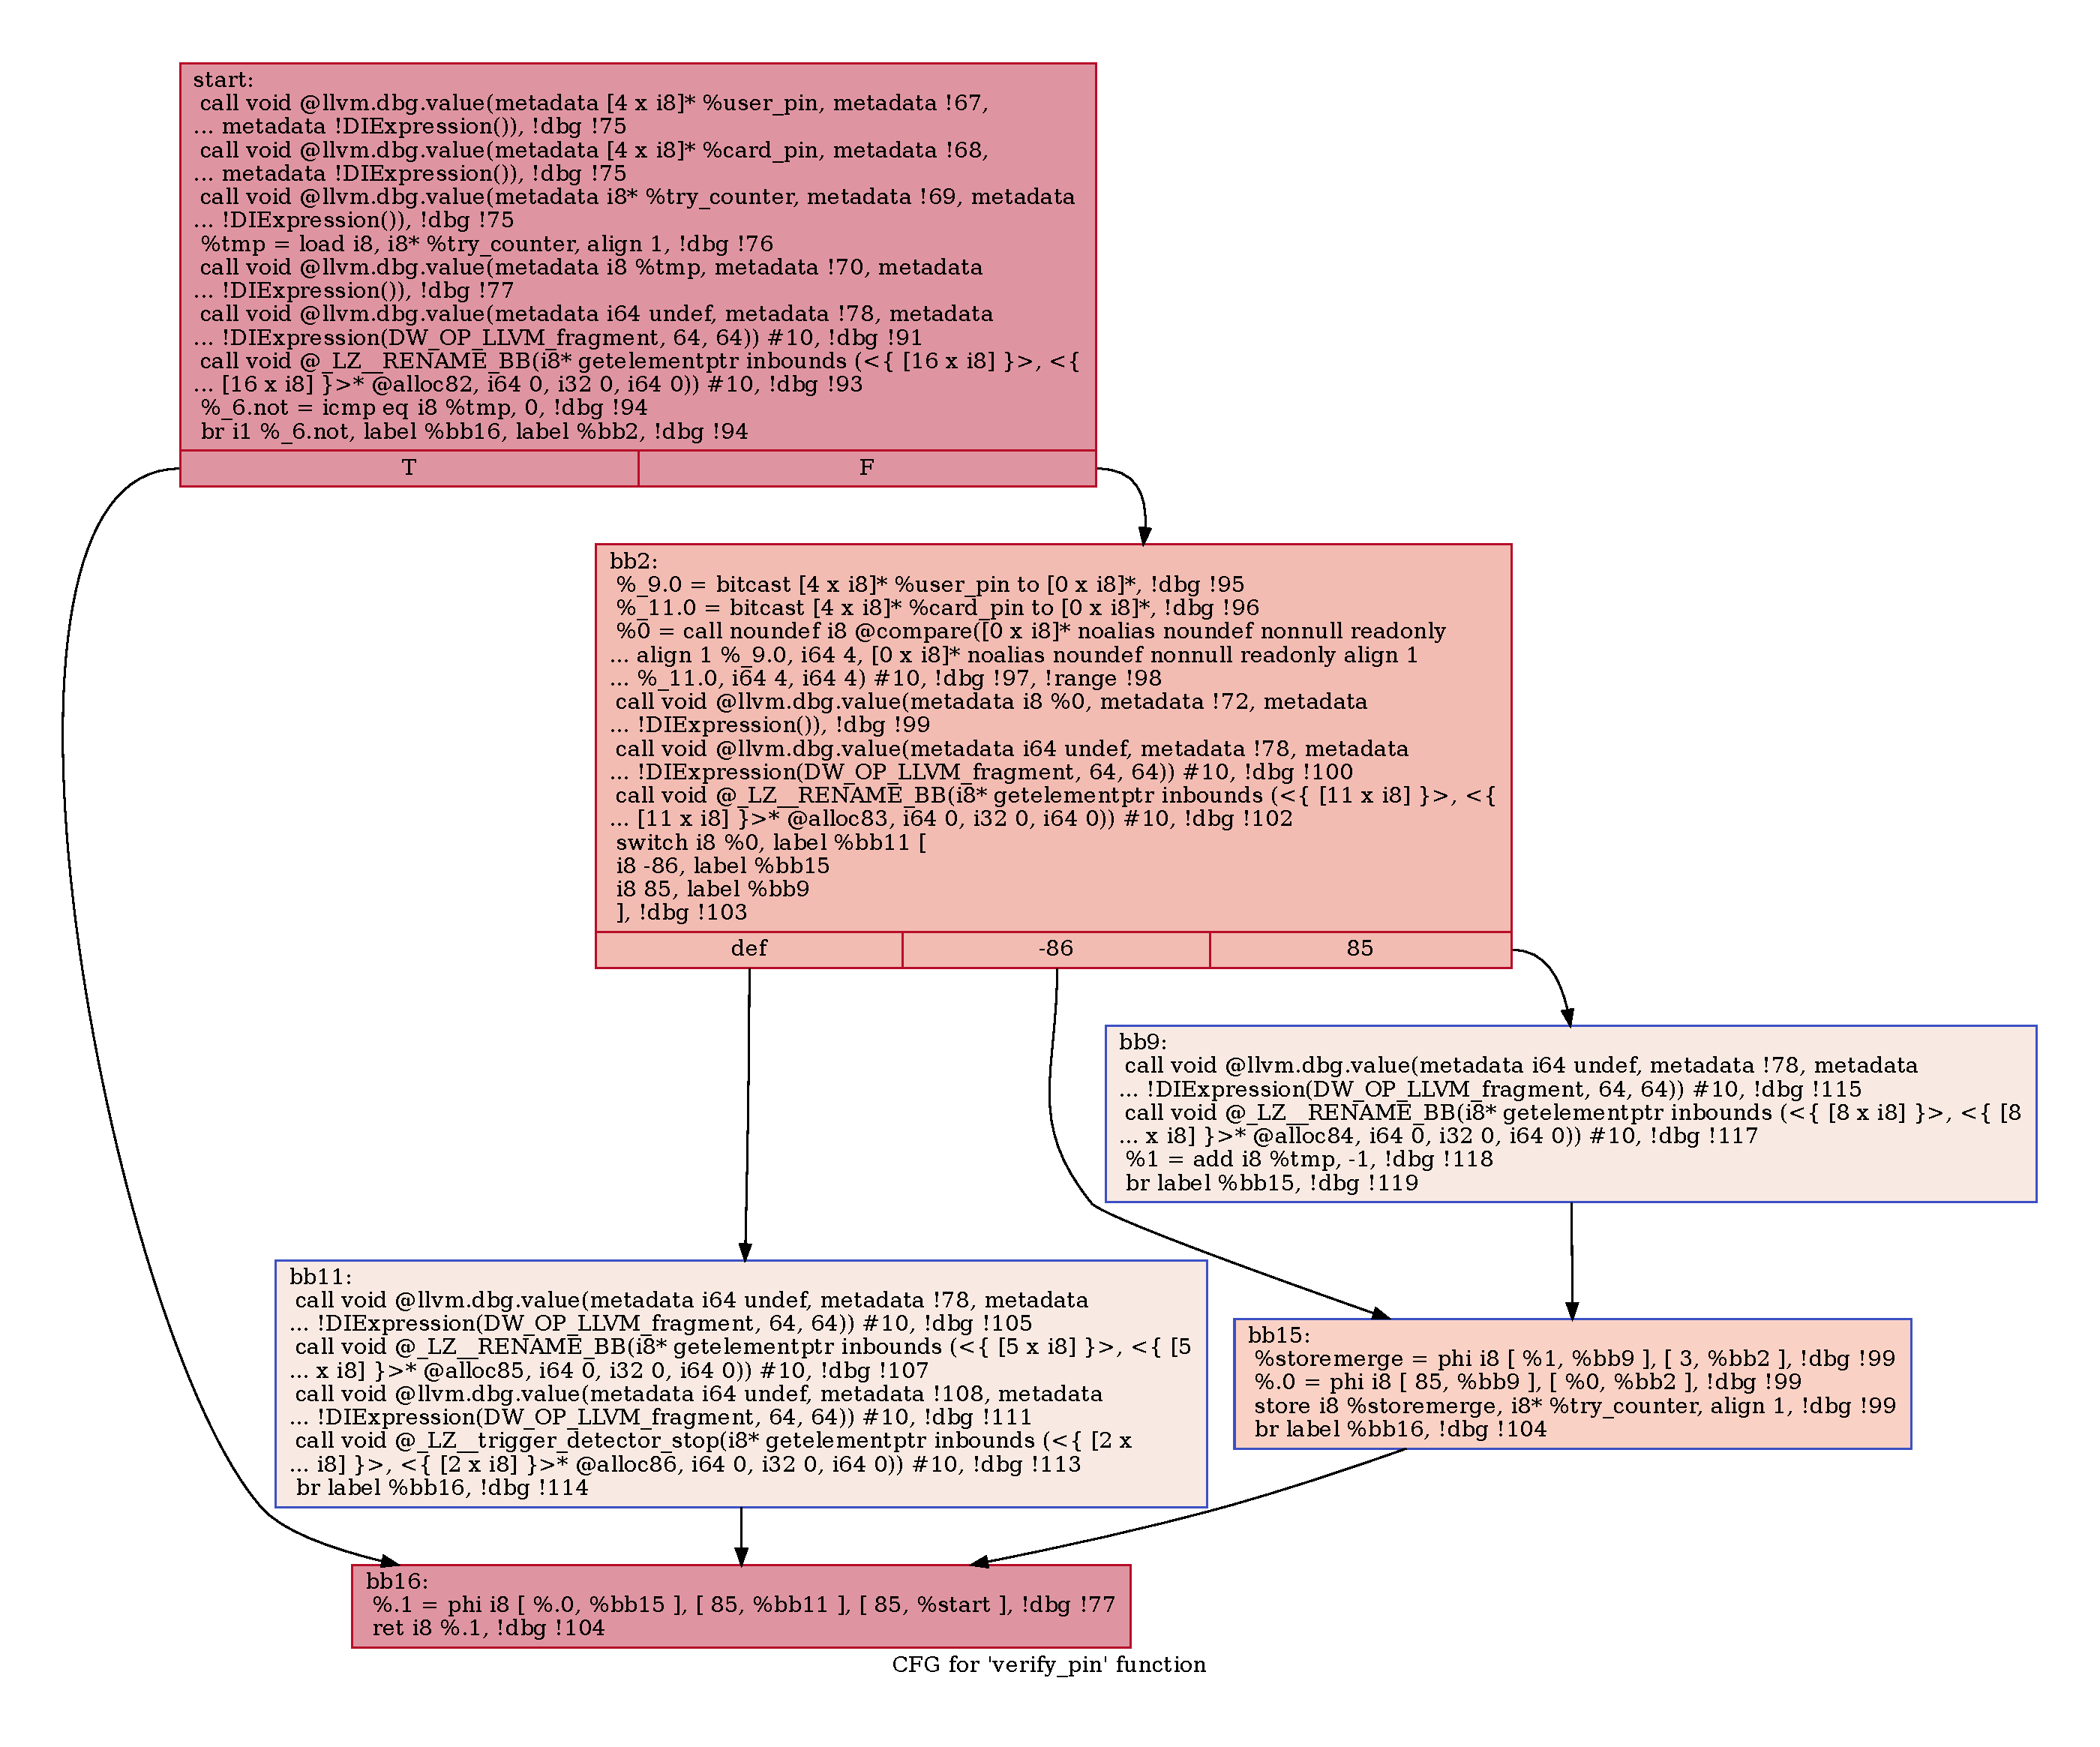
\includegraphics[width=1\textwidth]{image/cfg.verify_pin.pdf}
    \caption{verify\_pin control flow graph}
    \label{fig:annexe1}
\end{figure}

\end{document}